% Báo cáo mini-project ScholarLens — học phần Khai phá dữ liệu lớn và học máy.
% Biên dịch: XeLaTeX (Overleaf: Menu -> Compiler -> XeLaTeX; file latexmkrc đã đặt sẵn).
\documentclass{pkareport}
% Lệnh dùng chung cho báo cáo ScholarLens.
\newcommand{\code}[1]{\texttt{#1}}          % tên file, lệnh, biến
\newcommand{\mo}[1]{\texttt{scholarlens.#1}} % tên module
\newcommand{\RRF}{\mathrm{RRF}}
\newcommand{\BM}{\mathrm{BM25}}
\newcommand{\rank}{\mathrm{rank}}
% Bảng: cột chữ tự xuống dòng, căn trái
\newcolumntype{L}{>{\raggedright\arraybackslash}X}
\newcolumntype{P}[1]{>{\raggedright\arraybackslash}p{#1}}


% ---- Thông tin trang bìa (sửa tại đây) ----
\loaibaocao{MINI-PROJECT HỌC PHẦN\\KHAI PHÁ DỮ LIỆU LỚN VÀ HỌC MÁY}
\tendetai{HỆ THỐNG TRUY XUẤT VÀ HỎI ĐÁP BÀI BÁO KHOA HỌC ARXIV\\VỚI GRAPH RAG VÀ CHATBOT}
\phanbaocao{ScholarLens: tìm kiếm lai, đồ thị tri thức và LLM tự host}
\gvhd{PGS.TS Phạm Tiến Lâm}
\tennhom{Nhóm 2}
\nhom{%
  \textbf{Dương Khánh Linh} (nhóm trưởng) & MHV: 25800037\\
  Cao Đức Soạn & MHV: 25800041\\
  Triệu Minh Quang & MHV: 25800042\\
  Nguyễn Thành Dương & MHV: 25800030\\[4pt]}
\khoa{25}
\noithoigian{HÀ NỘI, 10/2026}
\logo{figures/logo_phenikaa.png}

\begin{document}
\taobia
\tableofcontents
\listoffigures
\listoftables
\begin{vietat}
\vt{API}{Application Programming Interface --- giao diện lập trình ứng dụng}
\vt{AWQ}{Activation-aware Weight Quantization --- lượng tử hóa trọng số có xét activation}
\vt{BM25}{Okapi Best Matching 25 --- hàm xếp hạng theo từ vựng}
\vt{CPU / GPU}{Bộ xử lý trung tâm / bộ xử lý đồ họa}
\vt{FR}{Functional Requirement --- yêu cầu chức năng}
\vt{HNSW}{Hierarchical Navigable Small World --- đồ thị nhiều tầng tìm láng giềng gần nhất xấp xỉ}
\vt{KG}{Knowledge Graph --- đồ thị tri thức}
\vt{LLM}{Large Language Model --- mô hình ngôn ngữ lớn}
\vt{MMR}{Maximal Marginal Relevance --- chọn kết quả vừa liên quan vừa đa dạng}
\vt{MRR}{Mean Reciprocal Rank --- trung bình nghịch đảo thứ hạng}
\vt{PDF}{Portable Document Format}
\vt{RAG}{Retrieval-Augmented Generation --- sinh câu trả lời có tăng cường truy xuất}
\vt{RRF}{Reciprocal Rank Fusion --- gộp xếp hạng theo nghịch đảo thứ hạng}
\vt{SHA-256}{Secure Hash Algorithm 256 bit --- hàm băm dùng kiểm tra trùng nội dung file}
\vt{SSE}{Server-Sent Events --- máy chủ đẩy sự kiện theo luồng qua HTTP}
\vt{UC}{Use Case --- tình huống sử dụng}
\vt{VRAM}{Bộ nhớ của GPU}
\end{vietat}

\chuongkhongso{TÓM TẮT}

Báo cáo trình bày \textbf{ScholarLens}, hệ thống truy xuất thông tin và hỏi đáp cho bài báo khoa học trên arXiv.
Người dùng tìm bài bằng câu hỏi tự nhiên (tiếng Việt hoặc tiếng Anh), thêm tài liệu bằng cách kéo-thả file PDF,
và trò chuyện với chatbot. Chatbot trả lời có trích dẫn tới đúng bài báo, kèm các bài liên quan tìm được trên đồ thị
tri thức.

Hệ thống gồm bảy module chạy độc lập: thu thập dữ liệu từ arXiv API; nạp PDF với ba lớp kiểm tra trùng (băm
SHA-256, mã arXiv, tiêu đề gần giống); embedding đa ngôn ngữ bằng \code{multilingual-e5-base} (tự dùng GPU); đồ thị
tri thức nối bài báo với tác giả, khái niệm, chuyên mục, quan hệ trích dẫn và tương đồng nội dung; chatbot hai chế
độ dựa trên Graph RAG; máy chủ LLM mã nguồn mở Qwen2.5 chạy bằng vLLM trên GPU Kaggle, công khai qua Cloudflare
Tunnel; và web app FastAPI có giao diện chat tối giản. Dữ liệu được tổ chức thành bốn kho: SQLite (metadata),
ChromaDB (vector, chỉ mục HNSW), chỉ mục BM25 và đồ thị NetworkX. Tìm kiếm kết hợp BM25 và vector bằng Reciprocal
Rank Fusion.

Trên kho thử nghiệm 492 bài, tìm bài theo tiêu đề bằng BM25 đạt Recall@1 = 0,957; cơ chế kiểm tra trùng phát hiện
95\% tiêu đề bị biến đổi mà không báo nhầm bài thật nào; trong năm bài liên quan mà đồ thị gợi ý, 37\% cùng chuyên
mục với bài gốc, gấp 2,7 lần so với chọn ngẫu nhiên.

\textbf{Từ khóa:} Information Retrieval, Hybrid Search, Graph RAG, Knowledge Graph, Chatbot, vLLM, arXiv.

\chapter{GIỚI THIỆU HỆ THỐNG}\label{chap:gioithieu}

\section{Đặt vấn đề}

ScholarLens là hệ thống truy xuất thông tin và hỏi đáp cho bài báo khoa học trên arXiv. Người dùng tìm bài bằng
câu hỏi tự nhiên (tiếng Việt hoặc tiếng Anh), thêm PDF bằng kéo-thả, và trò chuyện với chatbot. Chatbot trả lời
có trích dẫn tới đúng bài và đúng đoạn, kèm các bài liên quan tìm được trên đồ thị tri thức.

Hệ thống được xây dựng cho mini-project học phần Khai phá dữ liệu lớn và học máy, theo chủ đề tìm kiếm văn bản
khoa học. Dữ liệu thử nghiệm gồm 492 bài về truy xuất thông tin, RAG, đồ thị tri thức và mô hình ngôn ngữ.

\section{Mục tiêu}

Bảng~\ref{tab:muctieu} đối chiếu từng yêu cầu của đề bài với phần hệ thống đáp ứng và chương trình bày chi tiết.

\begin{table}[H]
\centering\small\setstretch{1.15}
\begin{tabularx}{\linewidth}{@{}P{0.28\linewidth}Lc@{}}
\toprule
\textbf{Yêu cầu của đề bài} & \textbf{ScholarLens đáp ứng bằng} & \textbf{Chương}\\
\midrule
Phát biểu bài toán, yêu cầu hệ thống & 7 tình huống sử dụng, 8 yêu cầu chức năng, 7 nhóm yêu cầu phi chức năng, yêu cầu môi trường sử dụng & 2, 3\\
Nguồn dữ liệu và cách thu thập & Crawler arXiv API (theo keyword, chuyên mục, mã bài), snapshot Kaggle, PDF người dùng tải lên & 4\\
Tổ chức hệ quản trị dữ liệu & SQLite + ChromaDB + chỉ mục BM25 + đồ thị tri thức; kiểm tra trùng ba lớp & 5\\
Hệ thống tìm kiếm đơn giản & Tìm kiếm lai BM25 + vector đa ngôn ngữ, gộp bằng RRF & 6\\
Tích hợp chatbot & Hai chế độ Chat / Research, Graph RAG, LLM Qwen2.5 tự host bằng vLLM & 7\\
Báo cáo kỹ thuật & Cấu trúc mã nguồn, triển khai, đánh giá, kiểm thử, hạn chế & 8\\
Trình bày giải pháp & Bộ slide 15 trang và kịch bản demo & 9\\
\bottomrule
\end{tabularx}
\caption{Đối chiếu yêu cầu của đề bài với hệ thống}\label{tab:muctieu}
\end{table}

\section{Kiến trúc tổng thể}

Hệ thống chạy trên hai máy (Hình~\ref{fig:kientruc}). Máy GPU (Kaggle, 2 GPU Tesla T4) làm phần tính toán nặng:
embedding hàng loạt và sinh câu trả lời bằng LLM. Máy demo chạy web app (trong Docker hoặc trực tiếp bằng Python),
giữ toàn bộ dữ liệu và phục vụ người dùng. Hai máy giao tiếp qua HTTPS bằng tunnel trycloudflare, có xác thực bằng
API key.

\begin{figure}[H]
\centering
% Sơ đồ kiến trúc tổng thể: máy GPU (Kaggle) và máy demo (Docker).
\begin{tikzpicture}[
  font=\footnotesize,
  box/.style={draw, rounded corners=2pt, align=center, text width=50mm, minimum height=11mm, fill=white,
    execute at begin node=\setstretch{1.05}},
  arr/.style={-{Stealth[length=2mm]}, thick},
  lbl/.style={font=\scriptsize, fill=white, inner sep=1pt}]
  % Máy GPU
  \node[box] (tun) at (0,0) {\textbf{cloudflared tunnel}\\https://\ldots.trycloudflare.com};
  \node[box, below=7mm of tun] (vllm) {\textbf{vLLM}: Qwen2.5-7B-Instruct-AWQ\\API tương thích OpenAI, 2 GPU};
  \node[box, below=7mm of vllm] (pipe) {\textbf{Pipeline dữ liệu (theo lô)}\\crawl $\to$ ingest $\to$ embedding $\to$ graph};
  % Máy demo
  \node[box] (web) at (8.0,0) {\textbf{Web app}\\FastAPI + giao diện chat};
  \node[box, below=7mm of web] (ret) {\textbf{Tìm kiếm lai + Graph RAG}\\BM25 + vector e5, gộp RRF};
  \node[box, below=7mm of ret] (store) {\textbf{Kho dữ liệu} \code{data/}\\SQLite, ChromaDB, BM25, đồ thị};
  \node[box, below=7mm of store] (emb) {\textbf{Embedder e5 (CPU)}\\embedding PDF mới tải lên};
  \node[box, above=9mm of web, text width=40mm, minimum height=8mm] (user) {Người dùng (trình duyệt)};
  % Khung hai máy
  \begin{scope}[on background layer]
    \node[draw, rounded corners=4pt, fill=black!4, inner sep=3.5mm, fit=(tun)(vllm)(pipe),
      label={[font=\small\bfseries]below:Máy GPU (Kaggle, 2$\times$T4)}] (gpu) {};
    \node[draw, rounded corners=4pt, fill=blue!4, inner sep=3.5mm, fit=(web)(ret)(store)(emb),
      label={[font=\small\bfseries]below:Máy demo (Docker hoặc Python)}] (demo) {};
  \end{scope}
  % Luồng
  \draw[arr] (user) -- (web);
  \draw[arr] (web) -- (ret);
  \draw[arr] (ret) -- (store);
  \draw[arr] (emb) -- (store);
  \draw[arr] (tun) -- (vllm);
  \draw[arr] (web.west) -- node[lbl, above]{HTTPS + API key} (tun.east);
  \draw[arr] (pipe.east) -- node[lbl, above]{chép \code{data/}} (store.west);
\end{tikzpicture}

\caption{Kiến trúc tổng thể của ScholarLens}\label{fig:kientruc}
\end{figure}

Câu hỏi đi từ trình duyệt vào web app, qua tìm kiếm lai và Graph RAG trên kho dữ liệu cục bộ. Chỉ bước sinh câu
trả lời đi qua tunnel tới vLLM. Pipeline dữ liệu chạy theo lô trên GPU, kết quả được chép sang máy demo một lần;
PDF thêm sau đó được embedding ngay trên máy demo.

\section{Công nghệ sử dụng}

\begin{table}[H]
\centering\small\setstretch{1.15}
\begin{tabularx}{\linewidth}{@{}P{0.25\linewidth}L@{}}
\toprule
\textbf{Tầng} & \textbf{Công nghệ}\\
\midrule
Thu thập, xử lý PDF & arXiv API~\cite{arxivapi}, PyMuPDF\\
Embedding & sentence-transformers~\cite{sbert}, \code{intfloat/multilingual-e5-base}~\cite{me5} (768 chiều, đa ngôn ngữ)\\
Lưu trữ & SQLite, ChromaDB 1.5.9 (chỉ mục HNSW~\cite{hnsw}), rank-bm25~\cite{bm25}, NetworkX~\cite{networkx}\\
LLM & vLLM~\cite{vllm} + Qwen2.5-7B-Instruct-AWQ~\cite{qwen25,awq}; có thể thay bằng Claude, Gemini, Ollama\\
Web app & FastAPI (streaming SSE), HTML/JS thuần, vis-network\\
Triển khai & Kaggle Notebook (GPU), Docker Compose, cloudflared\\
\bottomrule
\end{tabularx}
\caption{Công nghệ sử dụng theo từng tầng}\label{tab:congnghe}
\end{table}

\section{Kết quả chính}

\begin{itemize}
\item Kho 492 bài, 877 đoạn văn; đồ thị tri thức 5.598 nút và 8.258 cạnh.
\item Tìm bài theo tiêu đề bằng BM25 đạt Recall@1 = 0,957; một truy vấn tìm kiếm mất khoảng 0,3 giây trên CPU.
\item Kiểm tra trùng phát hiện 95\% tiêu đề bị biến đổi, không báo nhầm bài thật nào.
\item Trong năm bài liên quan mà đồ thị gợi ý, 37\% cùng chuyên mục với bài gốc, gấp 2,7 lần chọn ngẫu nhiên.
\end{itemize}

\section{Cấu trúc báo cáo}

Chương~\ref{chap:baitoan} phát biểu bài toán và các tình huống sử dụng. Chương~\ref{chap:yeucau} nêu yêu cầu chức
năng, phi chức năng và môi trường sử dụng. Chương~\ref{chap:dulieu} trình bày nguồn dữ liệu và cách thu thập.
Chương~\ref{chap:tochuc} mô tả tổ chức các kho dữ liệu và cơ chế kiểm tra trùng. Chương~\ref{chap:timkiem} trình
bày hệ thống tìm kiếm lai. Chương~\ref{chap:chatbot} trình bày chatbot và Graph RAG. Chương~\ref{chap:kythuat} là
báo cáo kỹ thuật: mã nguồn, triển khai, đánh giá, kiểm thử và hạn chế. Chương~\ref{chap:giaiphap} trình bày kịch
bản demo, kết luận và hướng phát triển.

\chapter{PHÁT BIỂU BÀI TOÁN}\label{chap:baitoan}

\section{Bài toán}

Cho một kho bài báo khoa học tăng dần theo thời gian, cần xây dựng hệ thống cho phép: (i) tìm đúng bài cần đọc
bằng câu hỏi tự nhiên; (ii) hỏi đáp về nội dung một bài cụ thể; (iii) khám phá các bài liên quan. Mọi câu trả lời
phải có dẫn nguồn kiểm chứng được.

arXiv nhận hơn 20.000 bài mới mỗi tháng. Tìm kiếm theo từ khóa đơn thuần bỏ sót các bài dùng thuật ngữ khác; còn
chatbot dùng LLM thuần túy dễ bịa nội dung và bịa trích dẫn. Vì vậy hệ thống cần kết hợp ba thành phần: truy xuất
theo ngữ nghĩa, quan hệ giữa các bài (tác giả, chủ đề, trích dẫn), và LLM để tổng hợp câu trả lời từ đúng các
đoạn văn tìm được (RAG~\cite{rag}).

\section{Tác nhân và tình huống sử dụng}

\begin{table}[H]
\centering\small\setstretch{1.15}
\begin{tabularx}{\linewidth}{@{}lP{0.17\linewidth}LL@{}}
\toprule
\textbf{Mã} & \textbf{Tác nhân} & \textbf{Tình huống} & \textbf{Kết quả mong đợi}\\
\midrule
UC1 & Học viên, nhà nghiên cứu & Tìm bài báo bằng câu hỏi tự nhiên, ví dụ ``retrieval augmented generation cho văn bản pháp luật'' & Danh sách bài xếp hạng, có tiêu đề, tác giả, năm, link arXiv\\
UC2 & Nhà nghiên cứu & Tải lên một file PDF bài báo & Hệ thống báo ``đã có'' hoặc tự xử lý và thêm vào kho\\
UC3 & Nhà nghiên cứu & Tải lên hàng loạt PDF & Mỗi file có trạng thái riêng: thêm mới, trùng hoặc lỗi\\
UC4 & Nhà nghiên cứu & Hỏi về một bài cụ thể (phương pháp, dữ liệu, kết quả) & Câu trả lời dựa trên các đoạn của chính bài đó, có trích dẫn [n]\\
UC5 & Nhà nghiên cứu & Hỏi ``các bài liên quan đến bài này'' & Danh sách bài láng giềng trên đồ thị kèm lý do liên quan\\
UC6 & Người dùng & Trò chuyện thông thường, hỏi khái niệm chung & Chế độ Chat trả lời nhanh, không truy xuất\\
UC7 & Quản trị viên & Thu thập dữ liệu theo keyword hoặc chuyên mục, embedding trên GPU & Kho dữ liệu được mở rộng\\
\bottomrule
\end{tabularx}
\caption{Tác nhân và tình huống sử dụng}\label{tab:usecase}
\end{table}

\section{Phạm vi}

Hệ thống tập trung vào bài báo khoa học trên arXiv, viết bằng tiếng Anh, ở dạng PDF hoặc metadata. Câu hỏi có thể
bằng tiếng Việt hoặc tiếng Anh. Hệ thống không xử lý ảnh, bảng hay công thức trong PDF như dữ liệu có cấu trúc;
chúng chỉ được đọc như văn bản thường.

\chapter{YÊU CẦU HỆ THỐNG}\label{chap:yeucau}

Yêu cầu được chia thành ba nhóm: chức năng (hệ thống phải làm gì), phi chức năng (làm tốt đến mức nào) và môi
trường sử dụng (cần gì để vận hành). Mỗi yêu cầu chức năng ứng với một module có thể chạy độc lập.

\section{Yêu cầu chức năng}

\begin{enumerate}[label=\textbf{FR\arabic*.}, leftmargin=3.2em]
\item \textbf{Thu thập:} lấy metadata và PDF từ arXiv API theo keyword, chuyên mục, khoảng ngày hoặc mã bài;
  không tải trùng.
\item \textbf{Nạp tài liệu:} nhận PDF, trích tiêu đề, tác giả, tóm tắt, mã arXiv và danh sách tài liệu tham khảo
  có mã arXiv.
\item \textbf{Kiểm tra trùng:} theo mã băm SHA-256 của file, mã arXiv, tiêu đề chuẩn hóa và tiêu đề gần giống.
\item \textbf{Embedding và lưu trữ:} chia đoạn, sinh vector, lưu vào vector DB và cập nhật đồ thị một cách tự
  động sau khi nạp.
\item \textbf{Tìm kiếm:} tìm kiếm lai BM25 + vector, gộp bằng Reciprocal Rank Fusion, lọc theo năm.
\item \textbf{Graph RAG:} mở rộng kết quả qua đồ thị (tác giả, chuyên mục, khái niệm, trích dẫn, tương đồng).
\item \textbf{Chatbot:} hai chế độ Chat và Research, trả lời có trích dẫn, ghi nhớ hội thoại, hỏi theo bài vừa
  thêm.
\item \textbf{Giao diện:} chat streaming, lịch sử hội thoại, kéo-thả PDF, danh sách nguồn và trực quan hóa đồ thị
  của từng câu trả lời.
\end{enumerate}

\section{Yêu cầu phi chức năng}

\begin{table}[H]
\centering\small\setstretch{1.15}
\begin{tabularx}{\linewidth}{@{}P{0.18\linewidth}LL@{}}
\toprule
\textbf{Nhóm} & \textbf{Yêu cầu} & \textbf{Cách đáp ứng}\\
\midrule
Hiệu năng & Tìm kiếm dưới 1 giây với kho 10.000 bài; nạp một PDF dưới 30 giây trên CPU & Chỉ mục HNSW (ChromaDB), BM25 trong bộ nhớ, embedding theo lô\\
Khả năng mở rộng & Embedding hàng chục nghìn bài & Chạy theo lô trên GPU Kaggle, xuất thư mục dữ liệu để dùng lại\\
Tính module & Mỗi module chạy độc lập & Gói Python \code{scholarlens.*}, mỗi module có lệnh riêng\\
Tính đúng đắn & Không bịa nguồn & Prompt buộc trích dẫn [n] từ ngữ cảnh; chế độ không LLM trả về trích đoạn\\
Tính linh hoạt & Đổi LLM hoặc model embedding & Cấu hình qua biến môi trường hoặc giao diện: API tương thích OpenAI (vLLM, Gemini, Ollama), Anthropic, hoặc không LLM\\
Tính khả dụng & Vẫn dùng được khi mất kết nối LLM & Tự quay về chế độ trích đoạn; tìm kiếm và đồ thị chạy cục bộ\\
Tính bảo trì & Dữ liệu tái lập được & Vector store và đồ thị dựng lại được toàn bộ từ SQLite\\
\bottomrule
\end{tabularx}
\caption{Yêu cầu phi chức năng}\label{tab:nfr}
\end{table}

\section{Yêu cầu môi trường sử dụng}

Máy demo không cần GPU. Mọi tính toán nặng nằm trên máy GPU, và máy GPU có thể là một phiên Kaggle miễn phí.

\begin{table}[H]
\centering\small\setstretch{1.15}
\begin{tabularx}{\linewidth}{@{}P{0.18\linewidth}LL@{}}
\toprule
\textbf{Thành phần} & \textbf{Yêu cầu tối thiểu} & \textbf{Cấu hình đã dùng khi phát triển}\\
\midrule
Máy GPU (LLM + embedding hàng loạt) & GPU NVIDIA có compute capability $\geq$ 7.5; tổng VRAM $\geq$ 16 GB cho model 7B nén AWQ ($\geq$ 8 GB cho model 3B); Linux, Python 3.10+, vLLM, có Internet & Kaggle Notebook, 2 $\times$ Tesla T4 (2 $\times$ 16 GB), Python 3.13, vLLM 0.32.0\\
Máy demo (web app) & CPU 4 nhân, RAM 8 GB, khoảng 3 GB ổ đĩa; Docker, hoặc Python 3.10+ & Windows 10, Python 3.13, chỉ CPU\\
Trình duyệt & Chrome, Edge hoặc Firefox bản hiện hành & Microsoft Edge\\
Mạng & Máy demo gọi ra ngoài qua HTTPS (tới tunnel trycloudflare, và arXiv API khi thêm PDF); không cần mở cổng vào & Mạng gia đình thông thường\\
Tài khoản & Kaggle đã xác minh để bật GPU và Internet; Hugging Face token nếu dùng model có giới hạn truy cập & Kaggle; Qwen2.5 không cần token\\
\bottomrule
\end{tabularx}
\caption{Yêu cầu môi trường sử dụng}\label{tab:moitruong}
\end{table}

Hai ràng buộc phải giữ đồng nhất giữa hai máy: cùng model embedding (\code{intfloat/multilingual-e5-base}) và cùng
phiên bản \code{chromadb} (1.5.9), để dữ liệu tạo trên máy GPU đọc được trên máy demo. Khi không có máy GPU, hệ
thống vẫn chạy ở chế độ trích đoạn: tìm kiếm, đồ thị và thêm PDF hoạt động bình thường, chỉ thiếu câu trả lời do
LLM viết.

\chapter{NGUỒN DỮ LIỆU VÀ PHƯƠNG THỨC THU THẬP}\label{chap:dulieu}

Dữ liệu là bài báo khoa học trên arXiv, thu thập qua ba kênh: arXiv API (theo keyword, chuyên mục, khoảng ngày
hoặc danh sách mã bài), bộ dữ liệu arXiv trên Kaggle, và PDF do người dùng tải lên. Tải file PDF là một tùy chọn
của kênh arXiv API, không phải kênh riêng. Bộ dữ liệu thử nghiệm gồm 492 bài, trong đó 12 bài có toàn văn PDF;
ngoài ra có 4 PDF được giữ riêng để trình diễn thao tác thêm bài.

\section{Các kênh thu thập}

\begin{table}[H]
\centering\small\setstretch{1.15}
\begin{tabularx}{\linewidth}{@{}P{0.2\linewidth}LP{0.17\linewidth}P{0.24\linewidth}@{}}
\toprule
\textbf{Kênh} & \textbf{Nội dung lấy được} & \textbf{Quy mô phù hợp} & \textbf{Lệnh}\\
\midrule
arXiv API~\cite{arxivapi} (Atom feed) & Mã bài, tiêu đề, tóm tắt, tác giả, chuyên mục, ngày, DOI, link PDF; tùy chọn tải PDF (toàn văn, mục, tài liệu tham khảo) & Vài nghìn bài mỗi truy vấn & \code{crawler keyword}, \code{crawler category}, \code{crawler ids}, cờ \code{--pdf}\\
Kaggle dataset Cornell-University/arxiv~\cite{arxivdataset} & Metadata của khoảng 2,7 triệu bài (JSON lines) & Hàng trăm nghìn bài & \code{crawler snapshot}\\
Người dùng tải lên & PDF bất kỳ, có hoặc không có mã arXiv; hệ thống tự tra metadata chuẩn trên arXiv API & Từng file hoặc theo lô & Giao diện web, \code{ingest pdf}, \code{ingest dir}\\
\bottomrule
\end{tabularx}
\caption{Các kênh thu thập dữ liệu}\label{tab:kenh}
\end{table}

\section{Phương thức thu thập}

\begin{enumerate}[label=(\arabic*)]
\item \textbf{Dựng truy vấn:} keyword được chuyển sang cú pháp arXiv. Cụm trong ngoặc kép thành
  \code{all:"..."}, từ rời được nối bằng AND; có thể ghép thêm chuyên mục \code{cat:cs.IR} và khoảng ngày
  \code{submittedDate:[từ TO đến]}.
\item \textbf{Thu thập không theo keyword:} lấy theo chuyên mục và khoảng ngày, ví dụ
  \code{crawler category cs.IR --from 2025-01-01}.
\item \textbf{Phân trang và tuân thủ quy định:} mỗi trang 100 kết quả, sắp xếp mới nhất trước; nghỉ tối thiểu
  3 giây giữa các lần gọi theo quy định của arXiv; thử lại khi lỗi mạng hoặc HTTP khác 200.
\item \textbf{Chống trùng khi thu thập:} kết quả được ghi nối vào \code{data/raw/metadata.jsonl}; mã bài đã có bị
  bỏ qua, nên thu thập lại nhiều lần không sinh bản sao.
\item \textbf{Tải PDF:} kiểm tra chữ ký \code{\%PDF} và kích thước file trước khi lưu vào \code{data/pdfs/}.
\end{enumerate}

Sau bước thu thập, bài báo chưa xuất hiện trong ứng dụng; cần chạy tiếp các bước nạp (\code{ingest}), embedding và
dựng đồ thị (Chương~\ref{chap:tochuc}).

\section{Bộ dữ liệu thử nghiệm}

\begin{table}[H]
\centering\small\setstretch{1.15}
\begin{tabularx}{\linewidth}{@{}Lr@{}}
\toprule
\textbf{Truy vấn thu thập} & \textbf{Số bài mới}\\
\midrule
12 bài kinh điển theo mã bài, kèm PDF (Transformer, BERT, RAG, DPR, REALM, FiD, Contriever, E5, BGE, Sentence-BERT, Self-RAG, RAPTOR) & 12\\
Keyword ``retrieval augmented generation'' & 150\\
Keyword ``dense retrieval'' & 97\\
Keyword ``graph neural network'', chuyên mục cs.LG & 80\\
Keyword ``knowledge graph'' question answering & 76\\
Chuyên mục cs.IR từ 01/2025 & 77\\
\midrule
\textbf{Tổng} & \textbf{492}\\
\bottomrule
\end{tabularx}
\caption{Thành phần bộ dữ liệu thử nghiệm}\label{tab:dataset}
\end{table}

Bốn PDF dành cho demo (không nạp sẵn): GraphRAG~\cite{graphrag} (2404.16130), RAG Survey (2312.10997),
LightRAG~\cite{lightrag} (2410.05779) và Agentic RAG Survey (2501.09136). Các file này được tải lại bằng
\code{scripts/download\_demo\_pdfs.py}.

\chapter{TỔ CHỨC HỆ QUẢN TRỊ DỮ LIỆU}\label{chap:tochuc}

Dữ liệu được chia vào bốn kho, mỗi kho phục vụ một kiểu truy vấn. SQLite là nguồn sự thật: ChromaDB, chỉ mục BM25
và đồ thị đều dựng lại được hoàn toàn từ SQLite. Cả bốn kho nằm trong một thư mục \code{data/}, nên có thể
embedding trên máy GPU rồi chép sang máy demo. Hình~\ref{fig:napdulieu} mô tả luồng nạp một PDF vào các kho.

\begin{figure}[H]
\centering
% Luồng nạp một PDF: ba lớp kiểm tra trùng trước khi ghi vào bốn kho dữ liệu.
% Lưới cột cố định (tâm cách nhau 3.8 cm), hộp rộng 3.0 cm -> không chồng nhau; tổng rộng ~14.4 cm.
\begin{tikzpicture}[
  font=\footnotesize,
  box/.style={draw, rounded corners=2pt, align=center, text width=27mm, minimum height=11mm, fill=white,
    execute at begin node=\setstretch{1.05}},
  gate/.style={box, fill=orange!12},
  store/.style={box, minimum height=9mm, fill=blue!6},
  dup/.style={box, text width=37mm, fill=black!6},
  arr/.style={-{Stealth[length=2mm]}, thick},
  lbl/.style={font=\scriptsize, fill=white, inner sep=1pt}]
  % Nhánh "đã có" (phía trên)
  \node[dup] (dup) at (7.6, 2.1) {\textbf{Đã có trong kho:} báo lý do,\\gắn bài cũ làm bài đang hỏi};
  % Hàng 1: chuỗi xử lý
  \node[box]  (pdf)   at (0.0, 0) {PDF tải lên\\(một hoặc nhiều file)};
  \node[gate] (sha)   at (3.8, 0) {\textbf{Lớp 1}\\trùng SHA-256?};
  \node[box]  (parse) at (7.6, 0) {Đọc PDF: tiêu đề,\\mã arXiv, refs};
  \node[gate] (id)    at (11.4, 0) {\textbf{Lớp 2}\\trùng mã / tiêu đề?};
  % Hàng 2: sau khi qua kiểm tra
  \node[gate] (api)   at (11.4, -2.1) {\textbf{Lớp 3}\\tra arXiv API, kiểm tra lại};
  \node[box]  (chunk) at (7.6, -2.1) {Chia đoạn\\220 từ, chồng 40};
  \node[box]  (emb)   at (3.8, -2.1) {Embedding\\+ trích khái niệm};
  % Hàng 3: bốn kho
  \node[store] (s1) at (0.0, -4.1) {SQLite};
  \node[store] (s2) at (3.8, -4.1) {ChromaDB};
  \node[store] (s3) at (7.6, -4.1) {BM25};
  \node[store] (s4) at (11.4, -4.1) {Đồ thị};
  \begin{scope}[on background layer]
    \node[draw, dashed, rounded corners=4pt, inner sep=2.5mm, fit=(s1)(s2)(s3)(s4),
      label={[font=\scriptsize\itshape]below:bốn kho dữ liệu trong thư mục \code{data/}}] (kho) {};
  \end{scope}
  % Luồng chính
  \draw[arr] (pdf) -- (sha);
  \draw[arr] (sha) -- node[lbl, above]{không} (parse);
  \draw[arr] (parse) -- (id);
  \draw[arr] (id) -- node[lbl, right]{không} (api);
  \draw[arr] (api) -- node[lbl, above]{mới} (chunk);
  \draw[arr] (chunk) -- (emb);
  \draw[arr] (emb.south) -- (emb.south |- kho.north);
  % Nhánh trùng
  \draw[arr] (sha.north) |- node[lbl, pos=0.25, left]{có} (dup.west);
  \draw[arr] (id.north) |- node[lbl, pos=0.25, right]{có} (dup.east);
\end{tikzpicture}

\caption{Luồng nạp một PDF: ba lớp kiểm tra trùng trước khi ghi vào bốn kho dữ liệu}\label{fig:napdulieu}
\end{figure}

\section{Bốn kho dữ liệu}

\begin{table}[H]
\centering\small\setstretch{1.15}
\begin{tabularx}{\linewidth}{@{}P{0.12\linewidth}P{0.24\linewidth}LL@{}}
\toprule
\textbf{Kho} & \textbf{Công nghệ} & \textbf{Nội dung} & \textbf{Phục vụ truy vấn}\\
\midrule
Metadata & SQLite (chế độ WAL), \code{scholarlens.sqlite} & Bảng \code{papers}, \code{chunks}, trạng thái pipeline & Kiểm tra trùng, lọc, chi tiết bài\\
Vector & ChromaDB 1.5 (HNSW~\cite{hnsw}, cosine), \code{chroma/} & Collection \code{chunks} (vector đoạn) và \code{papers} (vector tiêu đề + tóm tắt) & Tìm kiếm ngữ nghĩa, láng giềng tương đồng\\
Từ vựng & BM25 Okapi~\cite{bm25} (rank-bm25), trong RAM & Token của mọi đoạn đã embedding & Khớp thuật ngữ chính xác\\
Đồ thị & NetworkX~\cite{networkx} MultiDiGraph, \code{graph.json} & Nút paper, author, category, concept và 5 loại cạnh & Bài liên quan, quan hệ cho Graph RAG\\
\bottomrule
\end{tabularx}
\caption{Bốn kho dữ liệu và vai trò}\label{tab:kho}
\end{table}

\section{Lược đồ SQLite}

\begin{table}[H]
\centering\small\setstretch{1.15}
\begin{tabularx}{\linewidth}{@{}P{0.1\linewidth}LP{0.22\linewidth}@{}}
\toprule
\textbf{Bảng} & \textbf{Cột chính} & \textbf{Chỉ mục}\\
\midrule
\code{papers} & \code{paper\_id} (mã arXiv không có hậu tố phiên bản, hoặc \code{local:<sha12>}), \code{title}, \code{title\_norm}, \code{authors}, \code{abstract}, \code{categories}, \code{year}, \code{pdf\_path}, \code{file\_sha256}, \code{source}, \code{refs} (mã arXiv được trích dẫn), \code{keywords}, \code{status}, \code{n\_chunks} & \code{arxiv\_id}, \code{file\_sha256}, \code{title\_norm}, \code{status}\\
\code{chunks} & \code{chunk\_id} = \code{<paper\_id>::<idx>}, \code{kind} (summary / body), \code{section}, \code{page}, \code{text}, \code{embedded} & \code{paper\_id}, \code{embedded}\\
\bottomrule
\end{tabularx}
\caption{Lược đồ SQLite}\label{tab:sqlite}
\end{table}

Các cột dạng danh sách được lưu dưới dạng JSON. Mỗi bài đi qua các trạng thái
\code{registered} $\to$ \code{embedded} $\to$ \code{graphed}. Nhờ vậy từng module chạy lại độc lập được: module
embedding chỉ xử lý các đoạn có \code{embedded = 0}, còn bước dựng đồ thị chỉ lấy các bài đã embedding.

\section{Vector store}

Mỗi vector đoạn văn mang metadata \code{paper\_id}, \code{title}, \code{year}, \code{category}, \code{section},
\code{page}, \code{kind}. Metadata này cho phép lọc ngay trong ChromaDB, ví dụ chỉ tìm trong bài đang hỏi hoặc chỉ
lấy bài từ năm 2024 trở đi. Collection \code{papers} (một vector cho mỗi bài) dùng để tính cạnh SIMILAR\_TO: mỗi
bài nối tới tối đa 5 bài có cosine $\geq$ 0,75. Khi dựng toàn bộ đồ thị, độ tương đồng được tính chính xác bằng nhân
ma trận theo khối; khi thêm từng bài, hệ thống dùng truy vấn HNSW xấp xỉ cho nhanh.

\section{Đồ thị tri thức}

\begin{table}[H]
\centering\small\setstretch{1.15}
\begin{tabularx}{\linewidth}{@{}P{0.18\linewidth}P{0.2\linewidth}L@{}}
\toprule
\textbf{Cạnh} & \textbf{Từ $\to$ Đến} & \textbf{Cách sinh}\\
\midrule
CITES & paper $\to$ paper & Mã arXiv trong phần References của PDF; khi thêm bài mới, cạnh được nối cả hai chiều (bài mới trích dẫn bài cũ và bài cũ trích dẫn bài mới)\\
SIMILAR\_TO & paper $\to$ paper & Cosine giữa vector cấp bài, trọng số bằng cosine\\
WRITTEN\_BY & paper $\to$ author & Tác giả lấy từ arXiv API, tên chuẩn hóa làm khóa\\
MENTIONS & paper $\to$ concept & 6 khái niệm mỗi bài, trích bằng KeyBERT~\cite{keybert} rút gọn: ứng viên n-gram 1--3 từ, xếp theo cosine với vector bài, chọn đa dạng bằng MMR~\cite{mmr}\\
IN\_CATEGORY & paper $\to$ category & Chuyên mục arXiv, ví dụ cs.IR, cs.CL\\
\bottomrule
\end{tabularx}
\caption{Các loại cạnh trong đồ thị tri thức}\label{tab:canh}
\end{table}

\section{Kiểm tra trùng lặp}\label{sec:dedup}

Việc kiểm tra đi từ rẻ đến đắt và dừng ngay khi phát hiện trùng:

\begin{enumerate}[label=(\arabic*)]
\item \textbf{SHA-256 của file:} bắt lại đúng file đã tải lên trước đó, không cần đọc PDF.
\item \textbf{Mã arXiv:} đọc từ tem dọc bên lề trang 1, từ đường dẫn arxiv.org trên trang 1, hoặc từ tên file.
\item \textbf{Tiêu đề chuẩn hóa} (bỏ dấu, chữ thường, chỉ giữ chữ và số) khớp tuyệt đối.
\item \textbf{Tiêu đề gần trùng:} tỉ lệ ký tự giống nhau $\geq$ 0,92; hoặc đồng thời độ bao hàm từ
  $|A\cap B|/\min(|A|,|B|) \geq 0{,}9$ và hệ số Jaccard $|A\cap B|/|A\cup B| \geq 0{,}8$, với tiêu đề ngắn hơn có ít
  nhất 6 từ. Tiêu chí thứ hai bắt được trường hợp bỏ hoặc thêm vài từ, ví dụ ``(Extended Version)''.
\item \textbf{Kiểm tra lại sau khi tra arXiv API} với mã và tiêu đề chuẩn. Bước này bắt được PDF không có tem arXiv
  nhưng là bài đã có trong kho.
\end{enumerate}

Trên 492 bài, cơ chế này phát hiện 100\% bản trùng theo mã arXiv và 95\% tiêu đề bị biến đổi, không báo nhầm bài
thật nào (chi tiết ở Mục~\ref{sec:danhgia}).

\chapter{PHÁT TRIỂN HỆ THỐNG TÌM KIẾM}\label{chap:timkiem}

Tìm kiếm kết hợp hai tín hiệu bổ sung cho nhau. BM25 bắt đúng thuật ngữ hiếm (tên mô hình, tên bộ dữ liệu), còn
embedding đa ngôn ngữ bắt được cách diễn đạt khác và câu hỏi tiếng Việt. Hai danh sách kết quả được gộp bằng
Reciprocal Rank Fusion (RRF)~\cite{rrf}, rồi quy về cấp bài báo.

\section{Chia đoạn}

\begin{itemize}
\item \textbf{Đoạn tóm tắt} (chỉ số 0): tiêu đề + tóm tắt. Bài chỉ có metadata (không có PDF) vẫn tìm được nhờ
  đoạn này.
\item \textbf{Đoạn nội dung:} cửa sổ trượt 220 từ, chồng lấn 40 từ, không vượt qua ranh giới mục; mỗi đoạn mang
  số trang và tên mục để trích dẫn chính xác.
\item Phần References bị cắt khỏi nội dung cần chia đoạn, nhưng các mã arXiv trong đó được giữ lại làm cạnh CITES.
\end{itemize}

\section{Embedding}

\begin{table}[H]
\centering\small\setstretch{1.15}
\begin{tabularx}{\linewidth}{@{}P{0.22\linewidth}L@{}}
\toprule
\textbf{Thuộc tính} & \textbf{Giá trị}\\
\midrule
Model mặc định & \code{intfloat/multilingual-e5-base}~\cite{me5}: khoảng 278 triệu tham số, vector 768 chiều, hỗ trợ tiếng Việt\\
Tiền tố & \code{query:} cho câu hỏi, \code{passage:} cho văn bản; họ BGE dùng câu chỉ dẫn riêng, tự nhận theo tên model\\
Chuẩn hóa & Chuẩn L2, nên tích vô hướng giữa hai vector chính là cosine\\
Thiết bị & Tự chọn CUDA $\to$ MPS $\to$ CPU; trên GPU dùng số thực 16 bit và lô lớn gấp 4 lần\\
Chạy độc lập & \code{python -m scholarlens.embedding --device cuda}, chỉ xử lý các đoạn có \code{embedded = 0}\\
\bottomrule
\end{tabularx}
\caption{Cấu hình embedding}\label{tab:embedding}
\end{table}

\section{Tìm kiếm lai và gộp hạng}

\paragraph{BM25.} Mỗi đoạn văn $d$ được chấm điểm theo các từ $t$ của câu hỏi $q$:
\begin{equation}
\BM(q,d) = \sum_{t \in q} \mathrm{IDF}(t)\,\frac{f(t,d)\,(k_1+1)}{f(t,d) + k_1\bigl(1 - b + b\,\frac{|d|}{\mathrm{avgdl}}\bigr)},
\label{eq:bm25}
\end{equation}
trong đó $f(t,d)$ là số lần từ $t$ xuất hiện trong đoạn (điểm tăng chậm dần khi từ lặp lại nhiều),
$\mathrm{IDF}(t)$ cho từ hiếm điểm cao hơn từ phổ biến, $|d|/\mathrm{avgdl}$ phạt nhẹ đoạn dài hơn trung bình;
$k_1 = 1{,}5$, $b = 0{,}75$ (mặc định của rank-bm25). Văn bản được tách từ đơn giản: chữ thường, bỏ từ dừng.

\paragraph{Tìm kiếm dense.} Câu hỏi được embedding (tiền tố \code{query:}), ChromaDB trả về 50 đoạn có cosine cao
nhất, có thể kèm điều kiện lọc theo bài hoặc theo năm.

\paragraph{Gộp bằng RRF.} Hai danh sách top-50 được gộp chỉ dựa trên thứ hạng:
\begin{equation}
\RRF(d) = \sum_{r \in \{\mathrm{dense},\,\BM\}} \frac{1}{k + \rank_r(d)}, \qquad k = 60.
\label{eq:rrf}
\end{equation}
Đoạn đứng cao ở cả hai danh sách được cộng điểm từ cả hai. RRF chỉ dùng thứ hạng nên không cần chuẩn hóa thang
điểm giữa BM25 (không có giới hạn trên) và cosine (từ $-1$ đến $1$).

\paragraph{Quy về cấp bài báo.} Các đoạn được nhóm theo bài; điểm của bài bằng điểm đoạn cao nhất cộng
$0{,}3 \times$ tổng điểm các đoạn còn lại của bài đó. Bài có nhiều đoạn khớp được thưởng nhẹ, nhưng một đoạn rất
khớp vẫn quyết định thứ hạng.

\section{Truy cập tìm kiếm}

\begin{table}[H]
\centering\small\setstretch{1.15}
\begin{tabularx}{\linewidth}{@{}P{0.38\linewidth}L@{}}
\toprule
\textbf{Điểm truy cập} & \textbf{Mô tả}\\
\midrule
Khung chat (chế độ Research) & Mọi câu hỏi chuyên môn đều chạy tìm kiếm lai; các bài tìm được hiện thành danh sách nguồn dưới câu trả lời\\
\code{GET /api/search?q=...\&mode=hybrid} & API trả về danh sách bài, điểm, đoạn trích và thời gian xử lý; \code{mode} nhận \code{hybrid}, \code{dense} hoặc \code{bm25} để so sánh ba phương pháp\\
\code{GET /api/papers?q=...} & Lọc nhanh kho theo tiêu đề, tác giả hoặc mã bài\\
\bottomrule
\end{tabularx}
\caption{Các điểm truy cập tìm kiếm}\label{tab:truycap}
\end{table}

\chapter{TÍCH HỢP CHATBOT KẾT HỢP TÌM KIẾM VÀ HỎI ĐÁP}\label{chap:chatbot}

Chatbot có hai chế độ do hệ thống tự chọn. \textbf{Chat} trò chuyện tự do, không truy xuất. \textbf{Research} chạy
Graph RAG và bắt buộc trích dẫn [n]. Khi người dùng vừa thêm PDF, bài đó trở thành \emph{bài đang hỏi} (focus):
các câu hỏi tiếp theo được trả lời từ chính bài đó, kèm các bài láng giềng trên đồ thị.

\section{Luồng một lượt trả lời}

\begin{enumerate}[label=(\arabic*)]
\item \textbf{Định tuyến:} đang có bài focus thì chọn Research; câu chào hỏi ngắn (biểu thức chính quy, tối đa
  8 từ) thì chọn Chat; còn lại chọn Research.
\item \textbf{Viết lại câu hỏi:} LLM biến câu hỏi cuối thành một truy vấn tiếng Anh độc lập, thay các đại từ
  (``bài này'', ``phương pháp đó'') bằng đối tượng cụ thể trong lịch sử hội thoại.
\item \textbf{Truy xuất Graph RAG} (Mục~\ref{sec:graphrag}): trả về danh sách nguồn đánh số, mỗi nguồn là một bài
  báo kèm các đoạn trích, vai trò (focus, tìm thấy, liên quan) và lý do liên quan.
\item \textbf{Sinh câu trả lời streaming} với prompt hệ thống yêu cầu: chỉ dùng ngữ cảnh, ghi [n] sau mỗi khẳng
  định, nói rõ khi không đủ thông tin, trả lời bằng ngôn ngữ của người hỏi.
\item \textbf{Lưu hội thoại} kèm nguồn và đồ thị con để mở lại được từ thanh bên.
\end{enumerate}

Mỗi lượt được phát thành chuỗi sự kiện SSE \code{meta} $\to$ \code{status} $\to$ \code{query} $\to$ \code{sources}
$\to$ \code{token}\ldots{} $\to$ \code{done}. Nhờ đó giao diện hiển thị tiến trình và nguồn trước khi câu trả lời
xuất hiện, rồi hiện câu trả lời dần từng chữ.

\section{Graph RAG}\label{sec:graphrag}

Graph RAG mở rộng RAG~\cite{rag} thông thường bằng một bước đi trên đồ thị tri thức, theo tinh thần của
GraphRAG~\cite{graphrag} và LightRAG~\cite{lightrag} nhưng ở mức đơn giản hơn.

\begin{itemize}
\item \textbf{Không có focus:} tìm kiếm lai lấy 5 bài ``hạt giống'' (mỗi bài 2 đoạn). Ba bài đầu được mở rộng sang
  2 láng giềng trên đồ thị, hoặc 4 nếu câu hỏi có ý ``liên quan / tương tự / so sánh / trích dẫn''.
\item \textbf{Có focus:} tóm tắt của bài cùng 8 đoạn khớp nhất trong chính bài (lọc theo \code{paper\_id} trên cả
  ChromaDB và BM25), cộng 4--8 bài liên quan của nó trên đồ thị.
\item \textbf{Quan hệ trên đồ thị} được viết thành câu (``A trích dẫn B'', ``A bàn về: \ldots'') và đưa vào ngữ
  cảnh. Nhờ vậy LLM trả lời được câu hỏi về quan hệ mà từng đoạn văn riêng lẻ không chứa.
\end{itemize}

Điểm liên quan của bài $q$ với bài $p$ được cộng dồn theo các đường đi 1--2 bước trên đồ thị:
\begin{equation}
\mathrm{score}(p,q) = \mathbb{1}[\mathrm{CITES}] + \cos_{\mathrm{SIMILAR}}(p,q)
  + \sum_{e \in N(p) \cap N(q)} \frac{w_{\mathrm{type}(e)}}{\log_2\bigl(2 + \deg(e)\bigr)},
\label{eq:lienquan}
\end{equation}
với $w = 0{,}6$ cho tác giả chung, $0{,}45$ cho khái niệm chung và $0{,}05$ cho chuyên mục chung. Thực thể càng phổ
biến (bậc $\deg(e)$ cao) thì càng ít giá trị phân biệt nên bị chia nhỏ điểm. Bài chỉ có chung chuyên mục thì không
được tính là liên quan. Mỗi kết quả kèm danh sách lý do để hiển thị, ví dụ ``trích dẫn bài này; cùng khái niệm
dense retrieval''.

\section{Mô hình ngôn ngữ}

\begin{table}[H]
\centering\small\setstretch{1.15}
\begin{tabularx}{\linewidth}{@{}P{0.2\linewidth}P{0.3\linewidth}L@{}}
\toprule
\textbf{Backend} & \textbf{Cấu hình} & \textbf{Ghi chú}\\
\midrule
vLLM tự host & Giao diện (dòng ``LLM'' ở thanh bên) hoặc \code{SL\_LLM\_PROVIDER=openai}, \code{SL\_LLM\_BASE\_URL} & Module \mo{llm\_server} host model Hugging Face, mặc định Qwen2.5-7B-Instruct-AWQ~\cite{qwen25,awq} trên 2 GPU T4\\
Claude & \code{SL\_LLM\_PROVIDER=anthropic} & Mặc định \code{claude-opus-5-5}; tự chuyển sang model dự phòng khi bị từ chối\\
API tương thích OpenAI khác & Gemini, Groq, Ollama & Dùng chung một client\\
Không LLM & \code{SL\_LLM\_PROVIDER=none} & Chế độ trích đoạn: chọn câu khớp nhất trong từng nguồn và liệt kê bài liên quan\\
\bottomrule
\end{tabularx}
\caption{Các backend LLM được hỗ trợ}\label{tab:llm}
\end{table}

vLLM~\cite{vllm} quản lý bộ nhớ đệm attention theo từng trang nhỏ (PagedAttention), ghép nhiều yêu cầu vào cùng
một lượt tính và chia mỗi lớp của mô hình cho 2 GPU cùng tính (tensor parallelism). Lượng tử hóa AWQ~\cite{awq}
nén trọng số xuống 4 bit, đưa mô hình 7B từ khoảng 15 GB xuống khoảng 5 GB để vừa với 2 GPU T4. Trên T4 (không hỗ
trợ bf16), module tự chọn \code{float16} và chế độ \code{enforce-eager} để tiết kiệm VRAM.

\section{Vận hành LLM từ xa}

LLM chạy trên máy GPU và được gọi qua một tunnel công khai, nên hệ thống phải chịu được việc tunnel đổi địa chỉ
hoặc mất kết nối: URL trycloudflare đổi mỗi lần khởi động lại tunnel, và phiên Kaggle có thể bị ngắt.

\begin{table}[H]
\centering\small\setstretch{1.15}
\begin{tabularx}{\linewidth}{@{}P{0.24\linewidth}L@{}}
\toprule
\textbf{Cơ chế} & \textbf{Cách làm}\\
\midrule
Đổi LLM khi đang chạy & Dòng ``LLM'' ở cuối thanh bên; bấm vào để nhập Base URL và API key. Ứng dụng kiểm tra kết nối qua \code{/v1/models}, tự thêm \code{/v1}, tự lấy tên model và áp dụng ngay, không cần khởi động lại. Cấu hình lưu ở \code{data/llm\_config.json}\\
Hiển thị trạng thái & Chấm xanh/đỏ và tên model trên dòng ``LLM'', làm mới mỗi 60 giây\\
Bảo vệ endpoint & vLLM bật \code{--api-key}; yêu cầu không có đúng khóa bị từ chối (HTTP 401). Khóa cố định đặt trong Kaggle Secrets\\
Tự quay về khi mất kết nối & Khi LLM không phản hồi, chatbot báo rõ lý do rồi trả lời bằng chế độ trích đoạn, nên không bao giờ trả về câu trả lời trống\\
Giữ phiên, tự mở lại tunnel & Trên máy GPU, \code{keep\_alive} kiểm tra vLLM và URL công khai mỗi 2 phút; sau 2 lần lỗi liên tiếp thì mở tunnel mới và chỉ in URL mới sau khi đã gọi thử thành công\\
\bottomrule
\end{tabularx}
\caption{Cơ chế vận hành LLM từ xa}\label{tab:vanhanh}
\end{table}

Khi kiểm thử với tunnel trycloudflare thật, URL mới cần khoảng 69 giây mới gọi được vì DNS chưa kịp cập nhật.
Kiểm thử này cũng phát hiện Cloudflare chặn User-Agent mặc định của thư viện \code{urllib}; nếu không gửi
User-Agent riêng, \code{keep\_alive} sẽ tưởng tunnel đã chết và đổi URL liên tục.

\chapter{BÁO CÁO KỸ THUẬT}\label{chap:kythuat}

Mã nguồn gồm 8 gói Python, trong đó 7 gói chạy độc lập bằng \code{python -m scholarlens.<module>} và cùng dùng
chung thư mục \code{data/}. Phần nặng (embedding hàng loạt, chạy LLM) chạy trên máy GPU; máy demo chỉ cần CPU để
chạy web app và embedding từng PDF mới.

\section{Cấu trúc mã nguồn và các module}

\begin{table}[H]
\centering\small\setstretch{1.15}
\begin{tabularx}{\linewidth}{@{}P{0.15\linewidth}P{0.3\linewidth}L@{}}
\toprule
\textbf{Module} & \textbf{Tệp chính} & \textbf{Lệnh chạy độc lập (ví dụ)}\\
\midrule
\code{crawler} & \code{arxiv\_client.py} & \code{crawler keyword}, \code{crawler category}, \code{crawler ids}, \code{crawler snapshot}\\
\code{ingest} & \code{pdf\_parser.py}, \code{chunker.py}, \code{pipeline.py} & \code{ingest jsonl}, \code{ingest pdf}, \code{ingest dir}, \code{ingest all}\\
\code{embedding} & \code{embedder.py}, \code{pipeline.py} & \code{embedding --device cuda}, \code{embedding --rebuild}\\
\code{graph} & \code{knowledge\_graph.py}, \code{keywords.py}, \code{builder.py} & \code{graph build}, \code{graph stats}, \code{graph related <mã bài>}\\
\code{retrieval} & \code{hybrid.py}, \code{graph\_rag.py} & Dùng qua chatbot và web app\\
\code{chat} & \code{llm.py}, \code{prompts.py}, \code{chatbot.py} & \code{chat --mode research}\\
\code{llm\_server} & \code{server.py} & \code{llm\_server --preset qwen2.5-7b-awq --tunnel cloudflared}\\
\code{app} & \code{server.py}, \code{static/} & \code{app --port 7860}\\
\bottomrule
\end{tabularx}
\caption{Các module của ScholarLens}\label{tab:module}
\end{table}

\section{Triển khai}

\begin{enumerate}[label=(\arabic*)]
\item \textbf{Trên máy GPU (Kaggle, 2 GPU T4):} mã nguồn và dữ liệu được đóng gói thành Kaggle Dataset
  (\code{scripts/make\_kaggle\_bundle.py}). Notebook \code{kaggle\_llm\_server.ipynb} lần lượt embedding và dựng
  đồ thị, đóng gói thư mục \code{data/} để tải về, cài vLLM, chạy mô hình, mở tunnel và giữ phiên sống.
\item \textbf{Trên máy demo:} giải nén thư mục \code{data/}, chạy \code{python -m scholarlens.app} hoặc
  \code{docker compose up -d --build}, mở trình duyệt và dán URL tunnel cùng API key vào dòng ``LLM''.
\end{enumerate}

Image Docker dùng \code{python:3.11-slim} với torch bản CPU và đã tải sẵn model embedding, nên chạy được mà không
cần mạng để tải model; thư mục \code{data/} được gắn vào container nên dữ liệu không mất khi xóa container. Máy GPU
và máy demo phải dùng cùng model embedding, vì vector câu hỏi và vector trong kho phải nằm trong cùng không gian.

\section{Giao diện}

Giao diện được giữ tối giản (Hình~\ref{fig:giaodien}). Thanh bên thu gọn hoặc mở rộng được, chứa lịch sử hội thoại
và dòng kết nối LLM. Khung chat hiển thị câu trả lời dần từng chữ; dưới mỗi câu trả lời có danh sách nguồn thu gọn
và nút xem đồ thị của câu trả lời đó. Đồ thị mở được toàn màn hình (Hình~\ref{fig:dothi}); bấm vào từng nút để xem
chi tiết. PDF được thêm bằng nút đính kèm hoặc kéo-thả vào cửa sổ.

\begin{figure}[H]
\centering
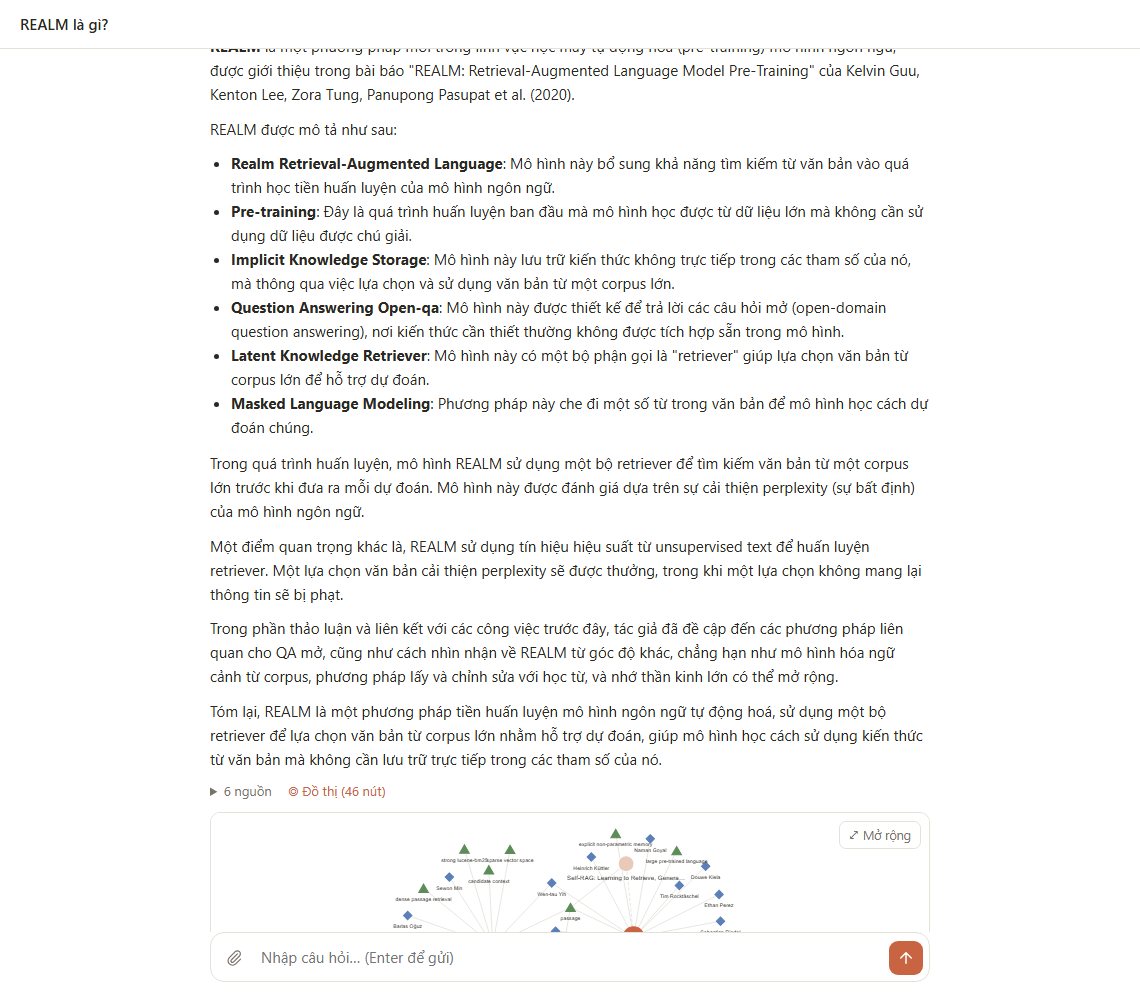
\includegraphics[width=0.85\linewidth]{figures/app_chat.png}
\caption{Khung chat: câu trả lời tiếng Việt có trích dẫn, danh sách nguồn và đồ thị của câu trả lời}\label{fig:giaodien}
\end{figure}

\begin{figure}[H]
\centering
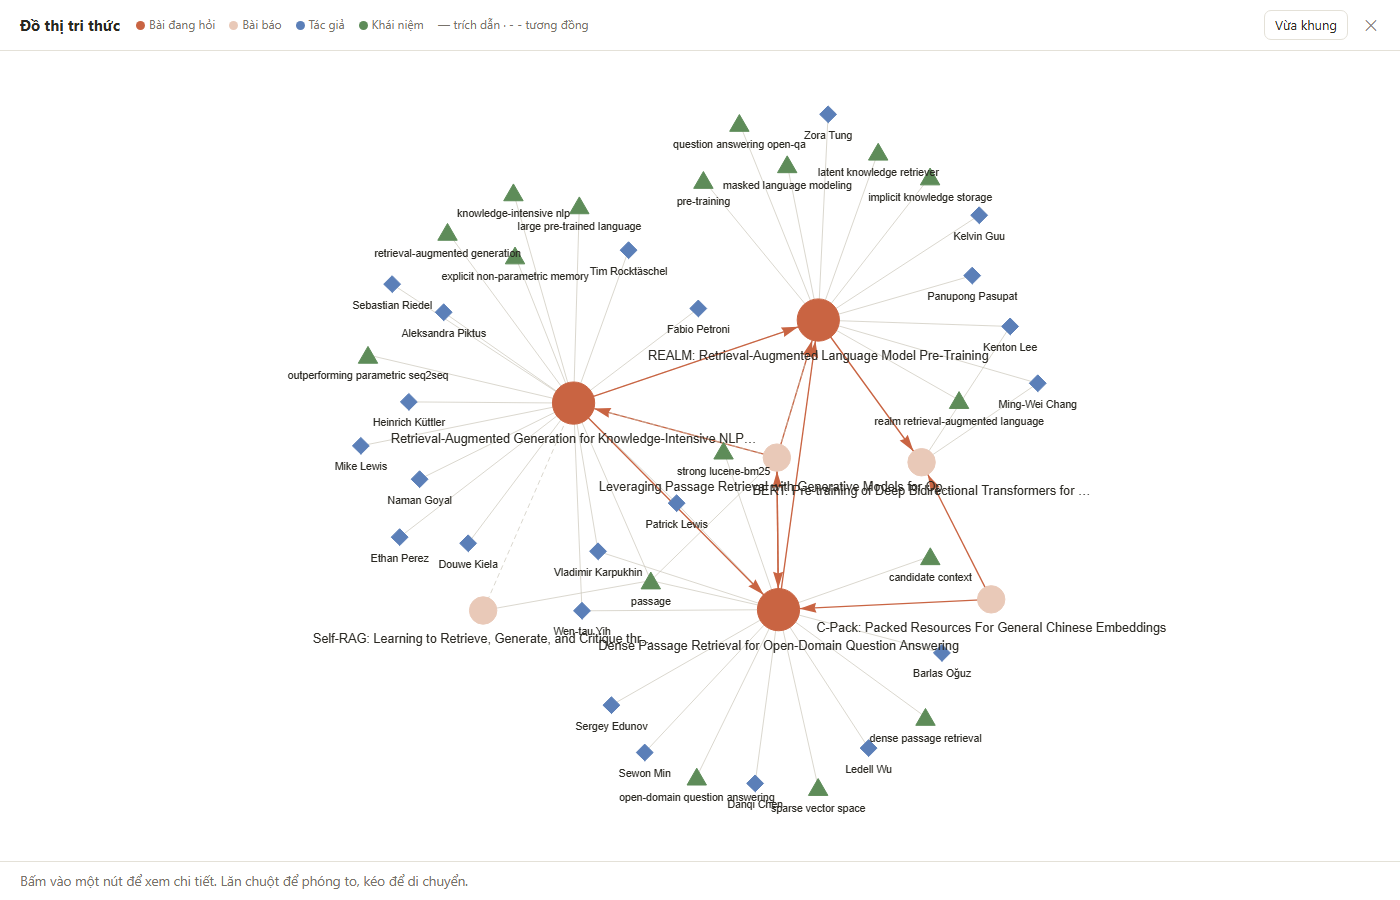
\includegraphics[width=\linewidth]{figures/app_graph_full.png}
\caption{Đồ thị toàn màn hình: bài đang hỏi (cam đậm), bài liên quan, tác giả, khái niệm và các cạnh trích dẫn}\label{fig:dothi}
\end{figure}

\section{Đánh giá}\label{sec:danhgia}

Script \code{scripts/evaluate.py} đo ba khía cạnh trên kho 492 bài:
\begin{itemize}
\item \textbf{Tìm bài theo tiêu đề (known-item):} truy vấn là tiêu đề, kho tìm kiếm là các tóm tắt không chứa tiêu
  đề, đáp án duy nhất là chính bài đó. Độ đo Recall@$k$ (tỉ lệ câu hỏi có đáp án nằm trong $k$ kết quả đầu) và
  MRR@10 (trung bình của $1/\text{hạng}$ của đáp án).
\item \textbf{Kiểm tra trùng:} 200 tiêu đề bị biến đổi ngẫu nhiên (chữ thường, bỏ dấu câu, bỏ một từ, thêm
  ``(Extended Version)''), cộng kiểm tra báo nhầm trên toàn bộ 492 tiêu đề thật.
\item \textbf{Đồ thị:} tỉ lệ bài liên quan (top-5) cùng chuyên mục chính với bài gốc, so với chọn ngẫu nhiên.
\end{itemize}

\begin{table}[H]
\centering\small\setstretch{1.15}
\begin{tabularx}{\linewidth}{@{}Lccccl@{}}
\toprule
\textbf{Phương pháp} & \textbf{R@1} & \textbf{R@5} & \textbf{R@10} & \textbf{MRR@10} & \textbf{Ghi chú}\\
\midrule
BM25 & 0,957 & 0,992 & 0,996 & 0,973 & 1,4 ms / truy vấn\\
Dense (multilingual-e5-base) & --- & --- & --- & --- & chưa chạy\\
Dense (bge-base-en-v1.5) & --- & --- & --- & --- & chưa chạy\\
Hybrid RRF (e5 + BM25) & --- & --- & --- & --- & chưa chạy\\
\bottomrule
\end{tabularx}
\caption{Kết quả tìm bài theo tiêu đề}\label{tab:knownitem}
\end{table}

BM25 đạt điểm rất cao vì từ của tiêu đề gần như luôn xuất hiện lại trong tóm tắt, nên bài kiểm tra này chủ yếu
xác nhận pipeline hoạt động đúng. Các dòng dense và hybrid cần chạy lại script trên GPU. Lợi ích của embedding thể
hiện rõ hơn ở câu hỏi tiếng Việt: trong kiểm thử chức năng, truy vấn ``phương pháp truy xuất dựa trên đồ thị cho
RAG'' đưa LightRAG lên hạng 1 dù chỉ có từ ``RAG'' trùng với văn bản tiếng Anh.

\begin{table}[H]
\centering\small\setstretch{1.15}
\begin{tabularx}{\linewidth}{@{}Lr@{}}
\toprule
\textbf{Kiểm tra trùng} & \textbf{Kết quả}\\
\midrule
Phát hiện theo mã arXiv & 100\% (200/200)\\
Phát hiện tiêu đề bị biến đổi & 95\% (190/200)\\
Báo nhầm trên 492 tiêu đề thật & 0\%\\
Báo nhầm với tiêu đề đối kháng (``<tiêu đề A> for X Revisited'') & 19\%\\
\bottomrule
\end{tabularx}
\caption{Kết quả kiểm tra trùng}\label{tab:dedup}
\end{table}

\begin{table}[H]
\centering\small\setstretch{1.15}
\begin{tabularx}{\linewidth}{@{}P{0.38\linewidth}L@{}}
\toprule
\textbf{Đồ thị tri thức} & \textbf{Kết quả}\\
\midrule
Quy mô & 5.598 nút (492 bài, 2.232 tác giả, 2.805 khái niệm, 69 chuyên mục), 8.258 cạnh\\
Cạnh theo loại & MENTIONS 2.952; WRITTEN\_BY 2.354; SIMILAR\_TO 2.052; IN\_CATEGORY 881; CITES 19\\
Bài có ít nhất một bài liên quan & 100\%\\
Bài liên quan (top-5) cùng chuyên mục & 37\% (chọn ngẫu nhiên: 14\%, tức gấp 2,7 lần)\\
\bottomrule
\end{tabularx}
\caption{Kết quả đánh giá đồ thị}\label{tab:graph}
\end{table}

Số cạnh CITES còn ít (19) vì chỉ 12 bài có toàn văn PDF; bài chỉ có metadata thì không có danh sách tài liệu
tham khảo.

\section{Kiểm thử chức năng}

\begin{table}[H]
\centering\small\setstretch{1.15}
\begin{tabularx}{\linewidth}{@{}P{0.4\linewidth}L@{}}
\toprule
\textbf{Kịch bản} & \textbf{Kết quả quan sát}\\
\midrule
Thêm PDF LightRAG (16 trang) & Tra arXiv API, 38 đoạn, 5 cạnh tương đồng, 6 khái niệm; khoảng 32 giây trên CPU\\
Thêm lại cùng file & Báo ``trùng nội dung file (SHA-256)'' ngay lập tức\\
Thêm PDF đã có từ bước thu thập (RAG, 2005.11401) & Báo ``trùng mã arXiv'' sau 0,2 giây\\
Tải lên hàng loạt 2 PDF qua web & Mỗi file một trạng thái riêng: 1 mới (6 bước), 1 trùng\\
Hỏi ``Tóm tắt bài này'' khi có bài focus & Chế độ Research, 5 nguồn, đồ thị con 17 nút\\
``xin chào'' & Định tuyến sang chế độ Chat\\
GraphRAG và LightRAG cùng trong kho & Tự sinh cạnh ``LightRAG trích dẫn GraphRAG'' từ References\\
Tunnel trycloudflare chết giữa chừng & \code{keep\_alive} tự mở tunnel mới; ứng dụng trả lời bằng chế độ trích đoạn trong lúc mất kết nối\\
\bottomrule
\end{tabularx}
\caption{Kết quả kiểm thử chức năng}\label{tab:kiemthu}
\end{table}

\section{Hạn chế}

\begin{itemize}
\item \textbf{Đọc PDF bằng quy tắc:} bảng, công thức và bố cục hai cột phức tạp có thể lộn thứ tự; tác giả trích
  từ PDF kém tin cậy khi không tra được arXiv API.
\item \textbf{Trích dẫn chỉ qua mã arXiv:} tài liệu tham khảo không ghi mã arXiv (bài hội nghị, tạp chí) chưa trở
  thành cạnh CITES.
\item \textbf{Khái niệm là n-gram:} đôi khi lấy cụm chung chung, làm giảm độ chính xác của cạnh MENTIONS.
\item \textbf{Embedding trên CPU chậm:} khoảng 1,4 đoạn/giây với e5-base, nên mỗi PDF mới mất chừng 30 giây khi
  demo trên máy không có GPU.
\item \textbf{Kiểm tra trùng với tiêu đề đối kháng:} tiêu đề mới chứa nguyên văn tiêu đề cũ cộng vài từ có thể bị
  báo trùng nhầm (19\% trong phép thử đối kháng).
\item \textbf{Ngôn ngữ của Qwen2.5:} mô hình đôi khi chuyển sang tiếng Trung giữa câu trả lời. Hệ thống đã thêm
  quy tắc ngôn ngữ vào prompt và lời nhắc trong từng lượt hỏi tiếng Việt; hiệu quả cần được theo dõi thêm.
\end{itemize}

\chapter{TRÌNH BÀY GIẢI PHÁP}\label{chap:giaiphap}

Phần trình bày dùng bộ slide \code{ScholarLens\_edited.pptx} (15 trang, có ghi chú người nói), sắp xếp theo đúng
các đề mục của báo cáo. Phần demo chạy trực tiếp trên web app với 4 PDF trong \code{demo\_pdfs/}; cả bốn bài chưa
có trong kho trước buổi demo.

\section{Kịch bản demo}

\begin{enumerate}[label=(\arabic*)]
\item \textbf{Chuẩn bị:} trên Kaggle chạy notebook \code{kaggle\_llm\_server.ipynb}; trên máy demo chạy
  \code{python -m scholarlens.app}, mở \code{http://127.0.0.1:7860}, dán URL trycloudflare và API key vào dòng
  ``LLM'' ở cuối thanh bên. Chấm xanh là sẵn sàng.
\item \textbf{Thêm một bài:} kéo file GraphRAG (\code{2404.16130.pdf}) vào cửa sổ. Tiến trình hiện ngay trong khung
  chat: SHA-256 $\to$ đọc PDF $\to$ tra arXiv API $\to$ chia đoạn $\to$ embedding $\to$ đồ thị. Kết thúc, dòng
  ``Đang hỏi về: \ldots'' xuất hiện phía trên ô nhập.
\item \textbf{Hỏi về bài:} ``Tóm tắt bài này'', ``Phương pháp chính và đóng góp là gì?''. Bấm một trích dẫn [n] để
  mở danh sách nguồn và tô sáng đúng bài đó.
\item \textbf{Hỏi bài liên quan:} ``Các bài báo liên quan đến bài này?'' cho danh sách kèm lý do (trích dẫn, cùng
  khái niệm, tương đồng nội dung). Bấm nút Đồ thị dưới câu trả lời, rồi Mở rộng để xem toàn màn hình và bấm vào một
  bài để xem chi tiết.
\item \textbf{Thêm trùng:} kéo lại cùng file; hệ thống báo ``đã có --- trùng nội dung file (SHA-256)'' và không
  embedding lại.
\item \textbf{Thêm hàng loạt:} chọn cùng lúc 3 PDF còn lại (RAG Survey, LightRAG, Agentic RAG); mỗi file hiện trạng
  thái riêng, rồi hỏi ``So sánh các bài vừa thêm''.
\item \textbf{Lịch sử và trình chiếu:} mở lại một hội thoại cũ trong thanh bên để cho thấy câu trả lời, nguồn và đồ
  thị được lưu lại; thu gọn thanh bên để khung chat chiếm toàn màn hình khi trình chiếu.
\end{enumerate}

\section{Kết luận}

ScholarLens đáp ứng đủ các yêu cầu của đề bài:
\begin{itemize}
\item Thu thập bài báo từ arXiv theo keyword, theo chuyên mục và theo mã bài, cùng nguồn snapshot Kaggle.
\item Tổ chức bốn kho dữ liệu (SQLite, ChromaDB, BM25, đồ thị) dựng lại được từ SQLite, với kiểm tra trùng ba lớp.
\item Tìm kiếm lai BM25 + vector đa ngôn ngữ gộp bằng RRF, hỏi được bằng tiếng Việt trên kho tiếng Anh.
\item Chatbot Graph RAG hai chế độ, trả lời có trích dẫn và gợi ý bài liên quan có giải thích.
\item LLM mã nguồn mở tự host bằng vLLM trên GPU miễn phí, chịu được việc mất kết nối.
\end{itemize}
Thao tác thêm PDF được tự động hóa trọn vẹn, kể cả kiểm tra trùng, và hệ thống vẫn chạy được khi không có LLM.

\section{Hướng phát triển}

\begin{table}[H]
\centering\small\setstretch{1.15}
\begin{tabularx}{\linewidth}{@{}P{0.36\linewidth}L@{}}
\toprule
\textbf{Hạn chế hiện tại} & \textbf{Hướng cải tiến}\\
\midrule
Đọc PDF bằng quy tắc & Dùng GROBID hoặc Nougat để lấy cấu trúc, bảng, công thức\\
Cạnh trích dẫn chỉ qua mã arXiv & Khớp tiêu đề tài liệu tham khảo, dùng Semantic Scholar API\\
Khái niệm dạng n-gram & Trích thực thể và quan hệ bằng LLM, tóm tắt cộng đồng như GraphRAG~\cite{graphrag} đầy đủ\\
Chưa có bước xếp hạng lại & Thêm cross-encoder (ví dụ bge-reranker) cho top-20 kết quả\\
Thu thập chạy thủ công & Theo dõi chủ đề định kỳ, chỉ lấy bài mới kể từ lần trước rồi tự nạp\\
Đánh giá known-item còn dễ & Xây bộ câu hỏi tiếng Việt có gán nhãn, đánh giá câu trả lời bằng LLM\\
\bottomrule
\end{tabularx}
\caption{Hạn chế và hướng phát triển}\label{tab:huongphattrien}
\end{table}

\begin{thebibliography}{99}

\bibitem{arxivapi}
arXiv: arXiv API User's Manual. \url{https://info.arxiv.org/help/api/user-manual.html}.

\bibitem{arxivdataset}
Clement, C.B., Bierbaum, M., O'Keeffe, K.P., Alemi, A.A.: On the use of arXiv as a dataset. arXiv:1905.00075
(2019).

\bibitem{bm25}
Robertson, S., Zaragoza, H.: The probabilistic relevance framework: BM25 and beyond. Foundations and Trends in
Information Retrieval 3(4), 333--389 (2009).

\bibitem{rrf}
Cormack, G.V., Clarke, C.L.A., Büttcher, S.: Reciprocal rank fusion outperforms Condorcet and individual rank
learning methods. In: Proceedings of the 32nd International ACM SIGIR Conference (2009).

\bibitem{hnsw}
Malkov, Y.A., Yashunin, D.A.: Efficient and robust approximate nearest neighbor search using Hierarchical
Navigable Small World graphs. IEEE Transactions on Pattern Analysis and Machine Intelligence 42(4), 824--836
(2020).

\bibitem{sbert}
Reimers, N., Gurevych, I.: Sentence-BERT: Sentence embeddings using Siamese BERT-networks. In: EMNLP-IJCNLP
(2019).

\bibitem{e5}
Wang, L., Yang, N., Huang, X., Jiao, B., Yang, L., Jiang, D., Majumder, R., Wei, F.: Text embeddings by
weakly-supervised contrastive pre-training. arXiv:2212.03533 (2022).

\bibitem{me5}
Wang, L., Yang, N., Huang, X., Yang, L., Majumder, R., Wei, F.: Multilingual E5 text embeddings: A technical
report. arXiv:2402.05672 (2024).

\bibitem{rag}
Lewis, P., Perez, E., Piktus, A., et al.: Retrieval-augmented generation for knowledge-intensive NLP tasks. In:
Advances in Neural Information Processing Systems (NeurIPS) (2020).

\bibitem{dpr}
Karpukhin, V., Oğuz, B., Min, S., et al.: Dense passage retrieval for open-domain question answering. In: EMNLP
(2020).

\bibitem{graphrag}
Edge, D., Trinh, H., Cheng, N., et al.: From local to global: A Graph RAG approach to query-focused
summarization. arXiv:2404.16130 (2024).

\bibitem{lightrag}
Guo, Z., Xia, L., Yu, Y., Ao, T., Huang, C.: LightRAG: Simple and fast retrieval-augmented generation.
arXiv:2410.05779 (2024).

\bibitem{keybert}
Grootendorst, M.: KeyBERT: Minimal keyword extraction with BERT. Zenodo (2020).

\bibitem{mmr}
Carbonell, J., Goldstein, J.: The use of MMR, diversity-based reranking for reordering documents and producing
summaries. In: Proceedings of the 21st International ACM SIGIR Conference (1998).

\bibitem{networkx}
Hagberg, A.A., Schult, D.A., Swart, P.J.: Exploring network structure, dynamics, and function using NetworkX. In:
Proceedings of the 7th Python in Science Conference (SciPy) (2008).

\bibitem{vllm}
Kwon, W., Li, Z., Zhuang, S., et al.: Efficient memory management for large language model serving with
PagedAttention. In: Proceedings of the 29th ACM Symposium on Operating Systems Principles (SOSP) (2023).

\bibitem{awq}
Lin, J., Tang, J., Tang, H., et al.: AWQ: Activation-aware weight quantization for on-device LLM compression and
acceleration. In: Proceedings of Machine Learning and Systems (MLSys) (2024).

\bibitem{qwen25}
Qwen Team: Qwen2.5 technical report. arXiv:2412.15115 (2024).

\end{thebibliography}

\end{document}
